\setcounter{secnumdepth}{6}
%%%%%%%%%%%%%%%%%%%%%%%%%%%%%%%%%%%%%%%%%%%
%%%%%%  STYLE 23
%%%%%%%%%%%%%%%%%%%%%%%%%%%%%%%%%%%%%%%%%%%
\newgeometry{left=4cm,right=4cm,bottom=2cm}

\cxset{style23/.style={
 name={Chapter},
 numbering=arabic,
 number font-size=\Large,
 number font-family=\rmfamily,
 number font-weight=\bfseries,
 number before={},
 number after={},
 number dot=,
 number position=rightname,
 chapter font-family=\sffamily,
 chapter font-weight=\normalfont,
 chapter font-size=\Large,
 chapter before={\hspace*{-50pt}\rule{\dimexpr\textwidth+50pt\relax}{0.4pt}\par\hspace*{-51pt}},
 chapter after={\par},
 chapter color={black!90},
 number color=\color{gray},
 title beforeskip={},
 title afterskip={\vspace{30pt}},
 title before=\hspace*{-50pt},
 title after={\par\vspace*{-10pt}\hspace*{-50pt}\rule{\dimexpr\textwidth+50pt}{0.4pt}\par},
 title font-family=\rmfamily,
 title font-color=\color{black!80},
 title font-weight=\bfseries,
 title font-size=\LARGE,
 section font-family=\rmfamily,
 section font-shape=\itshape,
 section font-weight=\bfseries,
 section numbering=arabic,
 section indent=-49pt,
 section beforeskip=\baselineskip,
 section afterskip=\baselineskip,
% subsection commands
 subsection font-shape=\upshape,
 subsection beforeskip=\baselineskip,
 subsection afterskip=10pt,
 subsection indent=-49pt,
 subsection numbering=arabic,
% subsection commands
 subsubsection font-family=\rmfamily,
 subsubsection font-shape=\itshape,
 subsubsection font-weight=\bfseries,
 subsubsection font-shape=\itshape,
 subsubsection font-size=\large,
 subsubsection align=,
 subsubsection beforeskip=10pt,
 subsubsection afterskip=\baselineskip,
 subsubsection indent=-49pt,
 subsubsection numbering=numeric,
% paragraphs
 paragraph font-family=\rmfamily,
 paragraph font-shape=\itshape,
 paragraph font-weight=\normalfont,
 paragraph font-shape=\itshape,
 paragraph font-size=\large,
 paragraph align=,
 paragraph beforeskip=10pt,
 paragraph afterskip=0pt,
 paragraph indent=-49pt,
 paragraph numbering=numeric,
% subparagraphs
 subparagraph font-family=\rmfamily,
 subparagraph font-shape=\itshape,
 subparagraph font-weight=\normalfont,
 subparagraph font-shape=\itshape,
 subparagraph font-size=\large,
 subparagraph align=,
 subparagraph beforeskip=10pt,
 subparagraph afterskip=0pt,
 subparagraph indent=-49pt,
 subparagraph numbering=arabic,
 subparagraph number after=\thinspace,
 header style=empty,
 pagestyle=headings,
}}


\cxset{headings style58}
\cxset{style23}
\chapter{Introduction to style twenty three}

\section{Introduction}

This style requires that the chapter settings as well as the
section headings are set in the margins, leaving the text after the sectioning commands to be indented. We achieve this by using negative skips.
\medskip
\begin{figure}[ht]
\centering
\fbox{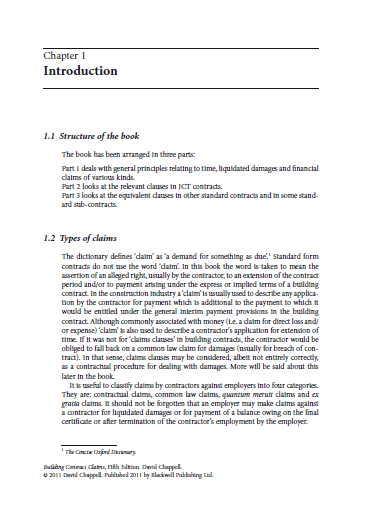
\includegraphics[width=0.45\textwidth]{./chapters/chapter23}
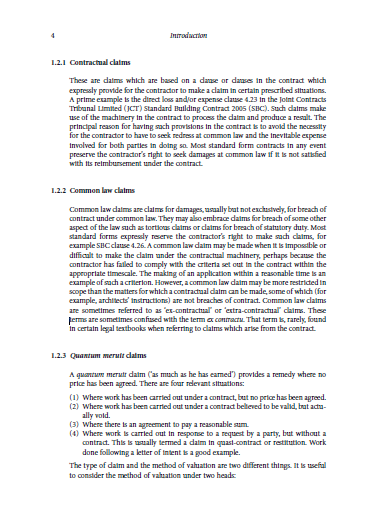
\includegraphics[width=0.45\textwidth]{./chapters/chapter23a}}
\end{figure}

\subsection{Subsections}
The same style is applied to the subsectioning commands up to the subsubsection which is not numbered but just uses an italic font. The subsubsection is also indented into the margin. Since the book is about construction claims it follows a style found in legal and construction documents, where all paragraphs are indented with respect to the section headings.
\lipsum[1-2]
\section{Even pages}
\lipsum[2]
\subsection{Setting different margins}
\lipsum[1]
\subsubsection{Setting Subsubsections}
\lipsum[1]
\paragraph{Paragraph level. } \lipsum*[3]\par

\lipsum[1]
\subparagraph{sub-paragraph level. } \lipsum*[3]\par


\restoregeometry
